\documentclass[article,type=msc,colorback,accentcolor=tud2a]{tudthesis}
%\documentclass[article,type=msc,colorback,accentcolor=tud2a]{tudreport}

%%%%%%%%%%%%%%%%%%%%%%%%%%%%%%%%%%%%%%%%%%%%%%%%%%%%%%%%%%%%%%%%%%%%%%%
%\usepackage{ngerman}

%%%%%%%%%%%%%%%%%%%%%%%%%%%%%%%%%%%%%%%%%%%%%%%%%%%%%%%%%%%%%%%%%%%%%%%

\newcommand{\getmydate}{%
  \ifcase\month%
    \or Januar\or Februar\or M\"arz%
    \or April\or Mai\or Juni\or Juli%
    \or August\or September\or Oktober%
    \or November\or Dezember%
  \fi\ \number\year%
}

\usepackage{masterthesis}

\begin{document}
\thesistitle{Implementation and Performance Analyses of a Highly Efficient Algorithm for Pressure-Velocity Coupling}{Implementierung und Untersuchung einer hoch effizienten Methode zur Druck-Geschwindigkeits-Kopplung}
%\title{Implementation and Performance Analyses of a Highly Efficient Algorithm for Pressure-Velocity Coupling}{Implementierung und Untersuchung einer hoch effizienten Methode zur Druck-Geschwindigkeits-Kopplung}
  \author{Fabian Gabel}
  \referee{Prof. Dr. rer. nat. Michael Schäfer}{Dipl.-Ing Ulrich Falk}
  \department{Studienbereich CE}
  \group{FNB}
% \tuprints{12345}{1234}
  \makethesistitle
% \maketitle
  \affidavit{F. Gabel}
  \tableofcontents

    %GEOMETRY
    \nomenclature{$x_i, i \in \{1,2,3\}$}{Cartesian coordinates}
    \nomenclature{$\vec{x}$}{Coordinate Vector}
    \nomenclature{$n_i, i \in \{1,2,3\}$}{Surface normal unit vector components}
    \nomenclature{$\vec{n}$}{Surface normal unit vector}
    \nomenclature{$t$}{Time}
    \nomenclature{$V$}{Volume}
    \nomenclature{$S$}{Surface}
    \nomenclature{$\left( \vec{e}_i \right)_{i=1,\dots,3}$}{Cartesian canonical basis}
    %PHYSICS
    \nomenclature{$\rho$}{Density}
    \nomenclature{$\mu$}{Dynamic viscosity}
    %\nomenclature{$\lambda$}{
    \nomenclature{$p$}{Pressure}
    \nomenclature{$u_i, i \in \{1,2,3\} $}{Cartesian velocity components}
    \nomenclature{$\vec{u}$}{Velocity vector}
    \nomenclature{$t_i, i \in \{1,2,3\}$}{Stress vector components}
    \nomenclature{$\vec{t}$}{Stress vector}
    \nomenclature{$k_i, i \in \{1,2,3\}$}{Mass specific force vector components}
    \nomenclature{$\vec{k}$}{Mass specific force vector}
    \nomenclature{$S_{ij}, i,j \in \{1,2,3\}$}{Symmetric part of the transpose of the jacobian of the velocity}
    \nomenclature{$\sigma_{ij}, i,j \in \{1,2,3\}$}{Deviatoric stress tensor}
    \nomenclature{$\tau_{ij}, i,j \in \{1,2,3\}$}{Coefficient matrix of stress mapping \(T\)}
    \nomenclature{$\vec{T}$}{Linear stress mapping}
    \nomenclature{$T$}{Temperature}
    \nomenclature{$\kappa$}{Thermal conductivity}
    \nomenclature{$q_T$}{Source or sink of heat}
    \nomenclature{$\rho_0$}{Reference density at \(T_0\)}
    \nomenclature{$T_0$}{Reference temperature}
    \nomenclature{$g_i, i \in \{1,2,3\}$}{Components of the gravitational acceleration vector}
    \nomenclature{$\vec{g}$}{Gravitational acceleration vector}
    \nomenclature{$\hat{p}$}{Pressure without hydrostatic pressure part}
    \nomenclature{$\beta$}{Coefficient of thermal expansion}
    %MATHEMATICS
    \nomenclature{$\delta_{ij}$}{Kronecker-Delta}
    %DIMENSIONLESS QUANTITIES
    \nomenclature{$Ma$}{Mach number}
    \printnomenclature



  \section{Introduction}

  This thesis is about. 

  \section{Fundamentals of Continuum Physics for Thermo-Hydrodynamical Problems}
\label{sec:fundamentals}

This section covers the set of fundamental equations for thermo-hydrodynamical problems which the numerical solution techniques of the following chapters are aiming to solve. Furthermore, the notation regarding the physical quantities to be used throughout this thesis is introduced. The following paragraphs are based on \cite{andersson84,ferziger02,kundu12,spurk10}. For a thorough derivation of the matter to be presented the reader may consult the mentioned sources. Since the present thesis focuses on the application of finite-volume methods, the focus lays on stating the integral forms of the relevant conservation laws. However, the process of deriving the final set of equations requires the use of differential formulations of the stated laws. Einstein's convention for taking sums over repeated indices simplifies certain expressions. The remainder of this thesis uses non-moving inertial frames in a Cartesian coordinate system with the coordinates \( x_i, i=1,...,3 \). This approach is also known as \emph{Eulerian approach}.  

\subsection{Conservation of Mass -- Continuity Equation}

The conservation law of mass, also known as the continuity equation, embraces the physical concept that, neglecting relativistic effects and nuclear reactions, mass cannot be created or destroyed. Using the notion of a mathematical control volume to denote a constant domain of integration, one can state the integral mass balance of a control volume \(V\) with control surface \(S\) with surface unit normal vector \(\vec{n} = \left( n_i \right)_{i=1,\dots,3}\) using Gauss's theorem as
\begin{displaymath}
  \iiint\limits_V \frac{\partial \rho}{\partial t} + \frac{\partial}{\partial x_i}\left( \rho u_i \right) \mathrm{d}V 
  =  \iiint\limits_V \frac{\partial \rho}{\partial t} \mathrm{d}V + \iint\limits_S \rho u_i n_i \mathrm{d}S
  = 0,
\end{displaymath}
where \( \rho \) denotes the material density, \(t\) denotes the independent variable of time and \(\vec{u} = \left( u_i \right)_{i=1,\dots,3}\) is the velocity vector field. Since this equation remains valid for arbitrary control volumes, the equality has to hold for the integrands as well. In this sense, the differential form of the conservation law of mass can be formulated as
\begin{equation}
  \label{eq:contifull}
  \frac{\partial \rho}{\partial t} + \frac{\partial}{\partial x_i}\left( \rho u_i \right)
  = 0.
\end{equation}

\subsection{Conservation of Momentum -- Cauchy-Equations}

The conservation law of momentum, also known as Newton's Second Law, axiomatically demands the balance of the temporal change of momentum and the sum of all attacking forces on a body. These forces can be divided into body forces and surface forces. Let \(\vec{k} = \left( k_i \right)_{i=1,\dots,3}\) denote a mass specific force and \(\vec{t} = \left(t_i\right)_{i=1,\dots,3}\) the stress vector. A first form of the integral momentum balance in the direction of \(x_i\) can be formulated as
\begin{equation}
\label{eq:cauchy}
\iiint\limits_V \frac{\partial }{\partial t}\left(\rho u_i \right) \mathrm{d}V + \iint\limits_S \rho u_i \left( u_j n_j \right) \mathrm{d}S = \iiint\limits_V \rho k_i \mathrm{d}V + \iint\limits_S t_i \mathrm{d}S.
\end{equation}

In general, the stress vector \(\vec{t}\) is a function not only of the location \(\vec{x} = \left( x_i \right)_{i = 1,\dots,3}\) and of the time \(t\) but also of the surface unit normal vector \(\vec{n}\). A central simplification can be introduced, namely Cauchy's stress theorem, which states that the stress vector is the image of the unit normal vector under a linear mapping \(\vec{T}\). With respect to the Cartesian canonical basis \(\left(\vec{e}_i \right)_{i = 1, \dots, 3}\), the mapping \(\vec{T}\) is represented by the coefficient matrix \( \left(\tau_{ji}\right)_{i,j = 1,\dots,3}\), and Cauchy's stress theorem reads
\begin{displaymath}
  \vec{t}\left(\vec{x},t,\vec{n}\right) = \vec{T}(\vec{x},t,\vec{n}) = \left(\tau_{ji} n_j\right)_{i = 1, \dots, 3}.
\end{displaymath}
Assuming the validity of Cauchy's stress theorem, one can derive Cauchy's first law of motion, which in differential form can be formulated as
\begin{equation}
  \label{eq:cauchymotion}
  \frac{\partial }{\partial t} \left(\rho u_i \right)
  + \frac{\partial}{\partial x_j}\left( \rho u_i u_j \right) 
  = \rho k_i + \frac{\partial \tau_{ji}}{\partial x_j}
\end{equation}
representing the starting point for the modeling of fluid mechanical problems. One should note that Cauchy's first law of motion does not make any assumptions regarding material properties, which is why the set of equations (\ref{eq:contifull},\ref{eq:cauchymotion}) is not closed, meaning that there does not exist an independent equation for each of the dependent variables.

%\subsection{Conservation of Angular Momentum}
\subsection{Closing the System of Equations -- Newtonian Fluids}
\label{sec:fundclosing}

As a result of Cauchy's theorem, the stress vector \( \vec{t} \) can be specified once the nine components \(\tau_{ji}\) of the coefficient matrix are known. As shown in \cite{kundu12,spurk10}, by formulating the conservation law of angular momentum the coefficient matrix is symmetric, 
\begin{equation}
  \label{eq:stresssymetry}
  \tau_{ji} = \tau_{ij},
\end{equation}
hence the number of unknown coefficients may be reduced to six unknown components. In a first step, it is assumed that the coefficient matrix can be decomposed into fluid-static and fluid-dynamic contributions,
\begin{displaymath}
  \tau_{ij} = -p \delta_{ij} + \sigma_{ij},
\end{displaymath}
where \(p\) is the thermodynamic pressure, \(\delta_{ij}\) is the \emph{Kronecker}-Delta and \( \sigma_{ij} \) is the so called \emph{deviatoric stress tensor}. 
    
In the present thesis, viscous fluids are modeled using a linear relation between the components of the deviatoric stress tensor and the symmetric part of the transpose of the Jacobian of the velocity field \(\left( S_{ij} \right)_{i,j=1,\dots,3}\),
\begin{displaymath}
  S_{ij} = \frac{1}{2} \left( \frac{\partial u_i}{\partial x_j} + \frac{\partial u_j}{\partial x_i} \right).
\end{displaymath}

If one now imposes material-isotropy and the mentioned stress-symmetry (\ref{eq:stresssymetry}) restriction, it can be shown \cite{aris62} that the constitutive equation for the deviatoric stress tensor reads 
\begin{displaymath}
  \sigma_{ij} = 2 \mu S_{ij} + \lambda S_{mm} \delta_{ij},
\end{displaymath}
where \(\lambda\) and \(\mu\) denominate scalars which depend on the local thermodynamical state. Taking everything into account, (\ref{eq:cauchymotion}) can be formulated as the differential conservation law of momentum for Newtonian fluids, better known as the \emph{Navier-Stokes equations} in differential form:
\begin{equation}
\label{eq:nsfull}
\frac{\partial }{\partial t} \left(\rho u_i \right)
+ \frac{\partial}{\partial x_j} \left( \rho u_i  u_j \right) 
= \rho k_i
- \frac{\partial p}{\partial x_i}
+ \frac{\partial}{\partial x_j} \left( \mu  \left( \frac{\partial u_i}{\partial x_j} 
                                        + \frac{\partial u_j}{\partial x_i} \right) \right)
+ \frac{\partial}{\partial x_i} \left(\lambda \frac{\partial u_m}{\partial x_m} \right)
\end{equation}

\subsection{Conservation of Scalar Quantities}

The modeling of the transport of scalar or vector quantities by a flow field \(\vec{u}\), also known as convection, is necessary if the fluid mechanical problem to be analyzed includes, for example, heat transfer. Other scenarios that involve the necessity to model scalar transport surge, when turbulent flows are to be modelled by two-equation models like the \(k\)-\(\varepsilon\)-model \cite{pope00}. 
    
Since this thesis focuses on the transport of the scalar temperature \(T\), this section introduces the conservation law of energy in differential form, formulated in terms of the temperature,
\begin{displaymath}
  \frac{\partial \left(\rho T \right)}{\partial t} + \frac{\partial}{x_j} \left( \rho u_j - \kappa \frac{\partial T}{\partial x_j} \right) = q_T,
\end{displaymath}
where \(\kappa\) denotes the thermal conductivity of the modelled material and \(q_T\) is a scalar field representing sources and sinks of heat throughout the domain of the problem. This equation is also known as the temperature equation.

        %Check also Peric p12 or Bird et al. (1962).

\subsection{Necessary Simplification of Equations}

The purpose of this section is to introduce and justify further common simplifications of the previously presented set of constitutive equations. 

\subsubsection{Incompressible Flows and Hydrostatic Pressure}

A common simplification when modeling low Mach number flows (\(Ma < 0.3\)), is the assumption of \emph{incompressibility}, or the assumption of an \emph{isochoric} flow. If one furthermore assumes homogeneous density \(\rho\) in space and time, a restrictive assumption that will be partially alleviated in the following section, the continuity equation in differential form (\ref{eq:contifull}) can be simplified to
\begin{displaymath}
  %\label{eq:contiinc}
  \frac{\partial u_i}{\partial x_i} = 0.
\end{displaymath}
In other words: In order for a velocity vector field \(\vec{u}\) to be valid for an incompressible flow, it has to be free of divergence, in other terms \emph{solenoidal} \cite{spurk10,aris62}.

If furthermore one assumes the dynamic viscosity \(\mu\) to be constant,  which can be suitable in the case of isothermal flow or if the temperature differences within the flow are small, the Navier-Stokes equations in differential form can be reduced to 
\begin{subequations}
\label{eq:navierstokes}
\begin{align}
  \frac{\partial}{\partial t}   \left(\rho u_i \right)
  + \rho \frac{\partial}{\partial x_j} \left( u_i  u_j \right) 
  =& \rho k_i
  - \frac{\partial p}{\partial x_i}
+ \frac{\partial}{\partial x_j} \left( \mu  \left( \frac{\partial u_i}{\partial x_j} 
+ \frac{\partial u_j}{\partial x_i} \right) \right) \\[0.5em]
  =& \rho k_i
  - \frac{\partial p}{\partial x_i}
  + \mu \frac{\partial}{\partial x_j} \left( \frac{\partial u_i}{\partial x_j} \right)
\end{align}
\end{subequations}
by using \emph{Schwartz}'s lemma to interchange the order of differentiation. Another common step to further simplify the set of equations is the assumption of a volume specific force \(\rho \vec{k}\) that can be modelled by a potential, in such a way that it can be represented as the gradient of a scalar field \(\Phi_\vec{k}\) as
\begin{displaymath}
 - \rho k_i = \frac{\partial \Phi_\vec{k}}{\partial x_i}.
\end{displaymath}

In the case of this thesis, this assumption is valid, since the mass specific force is the mass specific gravitational force \(\vec{g} = \left( g_i \right)_{i = 1,\dots,3}\), and the density is assumed to be constant, so that the potential can be modeled as
\begin{displaymath}
  \Phi_g = - \rho g_j x_j.
\end{displaymath}
This term can be interpreted as the hydrostatic pressure \(p_{hyd}\) and can be added to the thermodynamical pressure \(p\) to simplify calculations 
\begin{align*}
  \rho g_i - \frac{\partial p}{\partial x_i} 
  =& \frac{\partial}{\partial x_i} \left( \rho g_j x_j \right) - \frac{\partial p}{\partial x_i} \nonumber \\[0.5em]
  =& \frac{\partial}{\partial x_i} \left( \rho g_j x_j \right) - \frac{\partial}{\partial x_i}  \left(\hat{p} + p_{hyd} \right) \nonumber \\[0.5em]
  =& - \frac{\partial \hat{p}}{\partial x_i}.
\end{align*}
Since in incompressible fluids only pressure differences matter, this has no effect on the solution. After finishing the calculations \(p_{hyd}\) can be calculated and added to the resulting pressure \(\hat{p}\).

\subsubsection{Variation of Fluid Properties -- The Boussinesq Approximation}
\label{sec:boussinesq}

Modeling of an incompressible flow with heat transfer has to take into account that fluid properties, as for example density, change with varying temperature. If the variation of temperature is small, one can still assume constant density to maintain the structure of the advection and diffusion terms in (\ref{eq:nsfull}), and only consider changes of the density in the gravitational term. If linear variation of density with respect to temperature is assumed, this approximation is called \emph{Boussinesq} approximation \cite{gray76}. This approximation furthermore consists in assuming that all other fluid properties are constant and viscous dissipation can be neglected. In this case, the Navier-Stokes equations are formulated using a reference density \(\rho_0\) at the reference temperature \(T_0\) and the following temperature-dependent density \(\rho\)
\begin{displaymath}
  \rho \left( T \right) = \rho_0 \left( 1 - \beta \left( T - T_0 \right) \right).
\end{displaymath}
Here, \(\beta\) denotes the coefficient of thermal expansion. Using the Boussinesq approximation, the incompressible Navier-Stokes equations in differential form can be formulated as
\begin{align*}
  \rho_0 \frac{\partial \left( u_i \right)}{\partial t} 
  + \rho_0 \frac{\partial}{\partial x_j} \left( u_i  u_j \right) 
  =& \rho_0 g_i + \left(\rho - \rho_0 \right) g_i
  - \frac{\partial p}{\partial x_i}
  +  \mu \frac{\partial}{\partial x_j} \left( \frac{\partial u_i}{\partial x_j} 
  + \frac{\partial u_j}{\partial x_i} \right)  \\[0.5em]
  =& \frac{\partial}{x_i}\left(\rho_0 g_j x_j \right) 
  + \left(\rho - \rho_0 \right) g_i
  - \frac{\partial p}{\partial x_i}
  +  \mu \frac{\partial}{\partial x_j} \left( \frac{\partial u_i}{\partial x_j} 
  + \frac{\partial u_j}{\partial x_i} \right)  \\[0.5em]
  =& - \frac{\partial \hat{p}}{\partial x_i} 
  + \left(\rho - \rho_0 \right) g_i
  +  \mu \frac{\partial}{\partial x_j} \left( \frac{\partial u_i}{\partial x_j} 
  + \frac{\partial u_j}{\partial x_i} \right)  \\[0.5em]
  =& - \frac{\partial \hat{p}}{\partial x_i} 
  - \rho_0 \beta \left( T - T_0 \right) \, g_i
  +  \mu \frac{\partial}{\partial x_j} \left( \frac{\partial u_i}{\partial x_j} 
                                       + \frac{\partial u_j}{\partial x_i} \right) 
\end{align*}
using \(\rho \vec{g}\) as the mass specific force. 

\subsection{Final Form of the Set of Equations}

In the previous subsections different simplifications have been introduced, which will be used throughout the thesis. The final form of the set of equations to be used is thereby presented. As a further simplification, the modified pressure \(\hat{p}\) will be treated as \(p\), and since the use of the Boussinesq approximation replaces the variable \(\rho\) by a linear function of the temperature \(T\), the reference density \(\rho_0\) for the remainder of this thesis will be referred to as \(\rho\). It should be noted that incompressibility has been taken into account
\begin{subequations}
\label{eq:completeset}
\begin{align}
\label{eq:contidiff}
\frac{\partial u_i}{\partial x_i} =& 0. \\[1em]
\label{eq:momentumdiff}
\rho \frac{\partial \left( u_i \right)}{\partial t} 
+ \rho \frac{\partial}{\partial x_j} \left( u_i  u_j \right) 
=& - \frac{\partial p}{\partial x_i} 
- \rho \beta \left( T - T_0 \right)\, g_i
+  \mu \frac{\partial}{\partial x_j} \left( \frac{\partial u_i}{\partial x_j} 
+ \frac{\partial u_j}{\partial x_i} \right) \\[1em]
\label{eq:temperaturediff}
\frac{\partial \left(\rho T \right)}{\partial t} + \frac{\partial}{x_j} \left( \rho u_j T - \kappa \frac{\partial T}{\partial x_j} \right) =& q_T.
\end{align}
\end{subequations}

  \section{Finite-Volume Methods for Incompressible Flows -- Theoretical Basics}

This section deals with the fundamentals of the numerical solution via a finite-volume method of the formerly presented set of partial differential equations (\ref{eq:completeset}). The focus of this section is to provide an overview over the methods to be used in the present thesis. The information contained in this section is based on \cite{ferziger02,jasak96,schaefer99,muzaferja}. The overview starts by mentioning the different grid types to be used and the discretization techniques to be applied. On the basis of integral formulations of the equations to be solved, the therein contained integrals and differential operators have to be discretized. Since the accuracy of the default concepts for discretizing differential operators degrades with decreasing grid quality, this chapter furthermore presents different approaches to handle corrections for cases in which the cause of degrading grid quality is increased non-orthogonality. 
  
The goal of the finite-volume method is to provide linear algebraic equations which can be used to determine an approximate solution of a partial differential equation. This system of linear algebraic equations can be solved by means of algorithms to be presented in the end of this section. However since the Navier-Stokes equations are in general non-linear an intermediate step has to be taken, by linearizing the discrete equations. This leads to the need of an iteration process, the \emph{Picard iteration}, which will also be explained briefly.
      
\subsection{Numerical Grid}

In this subsection a brief overview of the general grid structure to be used in the present thesis is given. The main idea behind finite-volume methods is to solve partial differential equations by integrating them over the specified continuous problem domain and dividing this domain into a finite number of subdomains, the so called \emph{control volumes}. The result of the this finite partition of a continuous problem domain is called the numerical grid. The grid consists of a finite number of control volumes which represent the boundaries of a discrete domain of integration. Depending on whether the numerical solution of an equation is to be calculated on the boundary vertices or in the center of a grid cell, the variable arrangement is denoted to be vertex or cell center oriented. For the remainder of the present thesis it is assumed that the variables reside in the cell centers of the respective control volumes.

Another option to arrange variables specifically for algorithms that solve the Navier-Stokes equations is the so called \emph{staggering}. This method stores the variable values of different variables at different grid locations, which facilitates the interpolation of the respective values. As the methods of employed in the present thesis are intended to be generally applicable to complex geometries the cell centered non-staggered approach offers more flexibility.  Figure \ref{fig:cellvertex} shows the different variable arrangement options on a two dimensional grid.

\begin{figure}
   \label{fig:cellvertex}
    \subfigure{
    \begin{minipage}[1\width]{0.3\textwidth}%
      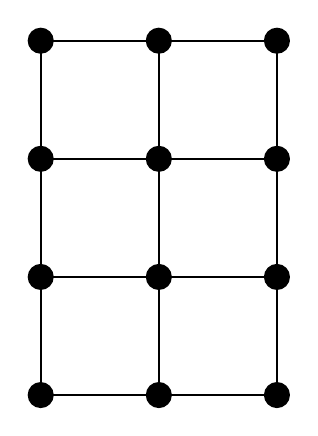
\begin{tikzpicture}

  \draw[thick] (0,0) rectangle (3,4.5);
  \draw[step=15mm,thick] (0,0) grid (3,4.5);

  \node at (0.0,0.0) [circle,fill=black] {};
  \node at (1.5,0.0) [circle,fill=black] {};
  \node at (3.0,0.0) [circle,fill=black] {};

  \node at (0.0  ,1.5) [circle,fill=black] {};
  \node at (1.5,1.5) [circle,fill=black] {};
  \node at (3.0,1.5) [circle,fill=black] {};

  \node at (0.0,3) [circle,fill=black] {};
  \node at (1.5,3) [circle,fill=black] {};
  \node at (3.0,3) [circle,fill=black] {};

  \node at (0.0,4.5) [circle,fill=black] {};
  \node at (1.5,4.5) [circle,fill=black] {};
  \node at (3.0,4.5) [circle,fill=black] {};


\end{tikzpicture}

      \raggedleft{}
    \end{minipage}}%
    \hfil
    \subfigure{
    \begin{minipage}[1\width]{0.3\textwidth}%
      \centering{}
      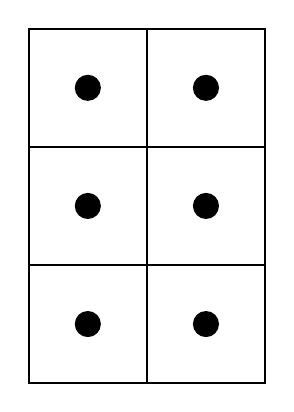
\begin{tikzpicture}

  \draw[thick] (0,0) rectangle (3,4.5);
  \draw[step=15mm,thick] (0,0) grid (3,4.5);

  \node at (0.75,0.75) [circle,fill=black] {};
  \node at (0.75,2.25) [circle,fill=black] {};
  \node at (0.75,3.75) [circle,fill=black] {};

  \node at (2.25,0.75) [circle,fill=black] {};
  \node at (2.25,2.25) [circle,fill=black] {};
  \node at (2.25,3.75) [circle,fill=black] {};

\end{tikzpicture}

    \end{minipage}}
    \hfil
    \subfigure{
    \begin{minipage}[1\width]{0.3\textwidth}%
      \raggedright{}
      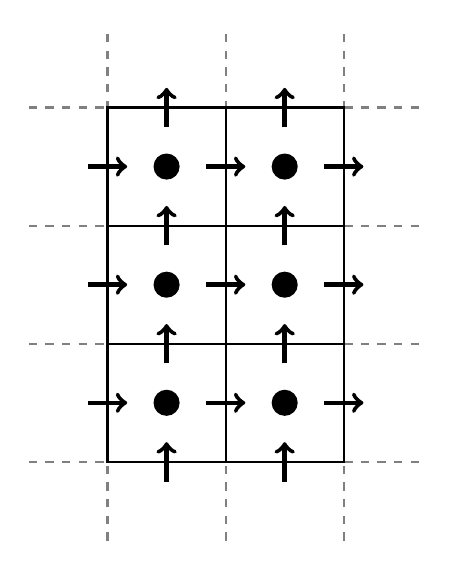
\begin{tikzpicture}

  \foreach \j in {-0.25,1.25,2.75,4.25} {
  \foreach \i in {0.75,2.25} {
    \draw[->,ultra thick] (\i,\j) -- (\i,\j+0.5){};
  } }

  \foreach \j in {0.75,2.25,3.75} {
  \foreach \i in {-0.25,1.25,2.75} {
    \draw[->,ultra thick] (\i,\j) -- (\i+0.5,\j){};
  } }

  \foreach \j in {0,1.5,3,4.5} {
    \draw[gray,thick,dashed] (-1.0,\j) -- (4.0,\j);
    }

  \foreach \i in {0,1.5,3} {
    \draw[gray,thick,dashed] (\i,-1.0) -- (\i,5.5);
    }

  \draw[thick] (0,0) rectangle (3,4.5);
  \draw[step=15mm,thick] (0,0) grid (3,4.5);

  \node at (0.75,0.75) [circle,fill=black] {};
  \node at (0.75,2.25) [circle,fill=black] {};
  \node at (0.75,3.75) [circle,fill=black] {};

  \node at (2.25,0.75) [circle,fill=black] {};
  \node at (2.25,2.25) [circle,fill=black] {};
  \node at (2.25,3.75) [circle,fill=black] {};


\end{tikzpicture}

    \end{minipage}}
    \caption{Vertex centered, cell centered and staggered variable arrangement}
\end{figure}

Regarding the treatment of domain boundaries and the ordering of the cells within the problem domain different types of numerical grids can be distinguished. The present thesis makes use of so called boundary fitted, block structured grids with hexahedron cells. A structured grid is characterized by a constant amount of of grid cells in each coordinate direction. The high regularity of structured grids benefits the computational efficiency of algorithms to be used on this type of grid. A block structured grid consists of different grid blocks of which each considered individually is structured, but if the topology of the grid is considered, it is unstructured. An example of a block structured grid with distinguishable grid blocks is given in figure \ref{fig:blockstruc}. The use of block structured grids is motivated by the need to increase the adaptivity of structured grids while maintaining high computational efficiency. Furthermore it naturally embraces the concept of domain decomposition which facilitates the implementation of parallel algorithms for the decomposed computational domain. Boundary fitted grids represent domain boundaries by means of the geometry of the control volumes residing on those boundaries. This approach may lead to skewed cells which furthermore affects the accuracy of the results obtained in these boundary cells. The mentioned affects can be alleviated by using local grid refinement techniques to refine the grid in regions of geometrically complex boundaries.

Inside a structured grid block, cells with the shape of hexahedrons are used. In addition to the geometric boundaries of each control volume a numerical grid also provides a mapping that assigns to each control volume with index \(P\) a set of indexes of neighbouring control volumes \(NB(P):=\{W,S,B,T,N,E\}\), which are named after the geographic directions. Figure \ref{fig:blockstruc} shows a single grid cell with its direct neighbours. The faces \(\{S_w,S_s,S,b,S_t,S_n,S_e\}\) of each hexahedral control volume represent the mentioned geometric boundaries. 

\begin{figure}[h]
  \label{fig:blockstruc}
  \subfigure{
  \begin{minipage}[1\width]{0.5\textwidth}%
    \begin{tikzpicture}
	\coordinate (P1) at (-25cm,6.5cm); % left vanishing point (To pick)
	\coordinate (P2) at (18cm,5.5cm); % right vanishing point (To pick)

	\coordinate (A1) at (0em,0cm); % central top point (To pick)
	\coordinate (A2) at (0em,1.5cm); % central bottom point (To pick)
	\coordinate (A3) at (0em,3cm); % central bottom point (To pick)

	\coordinate (A4) at ($(P1)!.94!(A1)$); 
	\coordinate (A5) at ($(P1)!.94!(A2)$);
	\coordinate (A6) at ($(P1)!.94!(A3)$);

	\coordinate (A7) at ($(P1)!.88!(A1)$); 
	\coordinate (A8) at ($(P1)!.88!(A2)$);
	\coordinate (A9) at ($(P1)!.88!(A3)$);

	\coordinate (A10) at ($(P2)!.94!(A1)$); 
	\coordinate (A11) at ($(P2)!.94!(A2)$);
	\coordinate (A12) at ($(P2)!.94!(A3)$);

	\coordinate (A19) at ($(P2)!.88!(A1)$); 
	\coordinate (A20) at ($(P2)!.88!(A2)$);
	\coordinate (A21) at ($(P2)!.88!(A3)$);

	\coordinate (A13) at
	  (intersection cs: first line={(A10) -- (P1)},
			    second line={(A4) -- (P2)});
	\coordinate (A14) at
	  (intersection cs: first line={(A11) -- (P1)}, 
			    second line={(A5) -- (P2)});
	\coordinate (A15) at
	  (intersection cs: first line={(A12) -- (P1)}, 
			    second line={(A6) -- (P2)});

	\coordinate (A16) at
	  (intersection cs: first line={(A10) -- (P1)},
			    second line={(A7) -- (P2)});
	\coordinate (A17) at
	  (intersection cs: first line={(A11) -- (P1)}, 
			    second line={(A8) -- (P2)});
	\coordinate (A18) at
	  (intersection cs: first line={(A12) -- (P1)}, 
			    second line={(A9) -- (P2)});

	\coordinate (A22) at
	  (intersection cs: first line={(A19) -- (P1)},
			    second line={(A4) -- (P2)});
	\coordinate (A23) at
	  (intersection cs: first line={(A20) -- (P1)}, 
			    second line={(A5) -- (P2)});
	\coordinate (A24) at
	  (intersection cs: first line={(A21) -- (P1)}, 
			    second line={(A6) -- (P2)});

	\coordinate (A25) at
	  (intersection cs: first line={(A19) -- (P1)},
			    second line={(A7) -- (P2)});
	\coordinate (A26) at
	  (intersection cs: first line={(A20) -- (P1)}, 
			    second line={(A8) -- (P2)});
	\coordinate (A27) at
	  (intersection cs: first line={(A21) -- (P1)}, 
			    second line={(A9) -- (P2)});

        \foreach \i in {1,2,3,4,5,6,7,8,9,
                        10,11,12,15,18,
                        19,20,21,24,27}
        {
	 %\draw[fill=black] (A\i) circle (0.15em) ;
        }

        %Vertical Lines
        \draw (A1) -- (A2) -- (A3);
        \draw (A4) -- (A5) -- (A6) -- (A15) -- (A24);
        \draw (A7) -- (A8) -- (A9) -- (A18) -- (A27);
        \draw (A12) -- (A15) -- (A18);
        \draw (A21) -- (A24) -- (A27);

        \fill[gray!30] (A1) -- (A19) -- (A21) -- (A3) -- cycle;
        %Horizontal Lines
        \draw (A7) -- (A4) -- (A1);
        \draw (A8) -- (A5) -- (A2);
        \draw (A9) -- (A6) -- (A3) -- (A12) -- (A21);
        \draw[gray,dashed] (A2) -- (A20);
        \draw[gray,dashed] (A10) -- (A12);
        \draw[gray,dashed] (A1) -- (A19);
        \draw[gray,dashed] (A19) -- (A21);

        %Boundary

	\coordinate (B1) at (0em,0cm);
	\coordinate (B2) at (0em,1cm);
	\coordinate (B3) at (0em,2cm);
	\coordinate (B4) at (0em,3cm);

	\coordinate (B5) at ($(P1)!1.05!(B1)$); 
	\coordinate (B6) at ($(P1)!1.05!(B2)$);
	\coordinate (B7) at ($(P1)!1.05!(B3)$);
	\coordinate (B8) at ($(P1)!1.05!(B4)$);

	\coordinate (B9)  at ($(P1)!1.1!(B1)$); 
	\coordinate (B10) at ($(P1)!1.1!(B2)$);
	\coordinate (B11) at ($(P1)!1.1!(B3)$);
	\coordinate (B12) at ($(P1)!1.1!(B4)$);

	\coordinate (B13)  at ($(P1)!1.15!(B1)$); 
	\coordinate (B14) at ($(P1)!1.15!(B2)$);
	\coordinate (B15) at ($(P1)!1.15!(B3)$);
	\coordinate (B16) at ($(P1)!1.15!(B4)$);

	\coordinate (B17) at ($(P2)!0.96!(B1)$); 
	\coordinate (B18) at ($(P2)!0.96!(B2)$);
	\coordinate (B19) at ($(P2)!0.96!(B3)$);
	\coordinate (B20) at ($(P2)!0.96!(B4)$);

        \coordinate (B33) at ($(P2)!.92!(B1)$); 
        \coordinate (B34) at ($(P2)!.92!(B2)$);
        \coordinate (B35) at ($(P2)!.92!(B3)$);
        \coordinate (B36) at ($(P2)!.92!(B4)$);

        \coordinate (B49) at ($(P2)!.88!(B1)$); 
        \coordinate (B50) at ($(P2)!.88!(B2)$);
        \coordinate (B51) at ($(P2)!.88!(B3)$);
        \coordinate (B52) at ($(P2)!.88!(B4)$);

	\coordinate (B21) at
	  (intersection cs: first line={(B17) -- (P1)},
			    second line={(B5) -- (P2)});
	\coordinate (B22) at
	  (intersection cs: first line={(B18) -- (P1)},
			    second line={(B6) -- (P2)});
	\coordinate (B23) at
	  (intersection cs: first line={(B19) -- (P1)},
			    second line={(B7) -- (P2)});
	\coordinate (B24) at
	  (intersection cs: first line={(B20) -- (P1)},
			    second line={(B8) -- (P2)});

	\coordinate (B25) at
	  (intersection cs: first line={(B17) -- (P1)},
			    second line={(B9) -- (P2)});
	\coordinate (B26) at
	  (intersection cs: first line={(B18) -- (P1)},
			    second line={(B10) -- (P2)});
	\coordinate (B27) at
	  (intersection cs: first line={(B19) -- (P1)},
			    second line={(B11) -- (P2)});
	\coordinate (B28) at
	  (intersection cs: first line={(B20) -- (P1)},
			    second line={(B12) -- (P2)});

	\coordinate (B29) at
	  (intersection cs: first line={(B17) -- (P1)},
			    second line={(B13) -- (P2)});
	\coordinate (B30) at
	  (intersection cs: first line={(B18) -- (P1)},
			    second line={(B14) -- (P2)});
	\coordinate (B31) at
	  (intersection cs: first line={(B19) -- (P1)},
			    second line={(B15) -- (P2)});
	\coordinate (B32) at
	  (intersection cs: first line={(B20) -- (P1)},
			    second line={(B16) -- (P2)});

	\coordinate (B37) at
	  (intersection cs: first line={(B33) -- (P1)},
			    second line={(B5) -- (P2)});
	\coordinate (B38) at
	  (intersection cs: first line={(B34) -- (P1)},
			    second line={(B6) -- (P2)});
	\coordinate (B39) at
	  (intersection cs: first line={(B35) -- (P1)},
			    second line={(B7) -- (P2)});
	\coordinate (B40) at
	  (intersection cs: first line={(B36) -- (P1)},
			    second line={(B8) -- (P2)});

	\coordinate (B41) at
	  (intersection cs: first line={(B33) -- (P1)},
			    second line={(B9) -- (P2)});
	\coordinate (B42) at
	  (intersection cs: first line={(B34) -- (P1)},
			    second line={(B10) -- (P2)});
	\coordinate (B43) at
	  (intersection cs: first line={(B35) -- (P1)},
			    second line={(B11) -- (P2)});
	\coordinate (B44) at
	  (intersection cs: first line={(B36) -- (P1)},
			    second line={(B12) -- (P2)});

	\coordinate (B45) at
	  (intersection cs: first line={(B33) -- (P1)},
			    second line={(B13) -- (P2)});
	\coordinate (B46) at
	  (intersection cs: first line={(B34) -- (P1)},
			    second line={(B14) -- (P2)});
	\coordinate (B47) at
	  (intersection cs: first line={(B35) -- (P1)},
			    second line={(B15) -- (P2)});
	\coordinate (B48) at
	  (intersection cs: first line={(B36) -- (P1)},
			    second line={(B16) -- (P2)});

	\coordinate (B53) at
	  (intersection cs: first line={(B49) -- (P1)},
			    second line={(B5) -- (P2)});
	\coordinate (B54) at
	  (intersection cs: first line={(B50) -- (P1)},
			    second line={(B6) -- (P2)});
	\coordinate (B55) at
	  (intersection cs: first line={(B51) -- (P1)},
			    second line={(B7) -- (P2)});
	\coordinate (B56) at
	  (intersection cs: first line={(B52) -- (P1)},
			    second line={(B8) -- (P2)});

	\coordinate (B57) at
	  (intersection cs: first line={(B49) -- (P1)},
			    second line={(B9) -- (P2)});
	\coordinate (B58) at
	  (intersection cs: first line={(B50) -- (P1)},
			    second line={(B10) -- (P2)});
	\coordinate (B59) at
	  (intersection cs: first line={(B51) -- (P1)},
			    second line={(B11) -- (P2)});
	\coordinate (B60) at
	  (intersection cs: first line={(B52) -- (P1)},
			    second line={(B12) -- (P2)});

	\coordinate (B61) at
	  (intersection cs: first line={(B49) -- (P1)},
			    second line={(B13) -- (P2)});
	\coordinate (B62) at
	  (intersection cs: first line={(B50) -- (P1)},
			    second line={(B14) -- (P2)});
	\coordinate (B63) at
	  (intersection cs: first line={(B51) -- (P1)},
			    second line={(B15) -- (P2)});
	\coordinate (B64) at
	  (intersection cs: first line={(B52) -- (P1)},
			    second line={(B16) -- (P2)});


        %Front lines
        \draw (B13) -- (B29) -- (B45) -- (B61);
        \draw (B1) -- (B5) -- (B9) -- (B13);
        \draw (B2) -- (B6) -- (B10) -- (B14);
        \draw (B3) -- (B7);
        \draw (B14) -- (B62);

        %Vertical lines
        \draw (B5) -- (B6) -- (B7) -- (B8);
        \draw (B29) -- (B30);
        \draw (B45) -- (B46) -- (B47) -- (B48);
        \draw (B61) -- (B62) -- (B63) -- (B64);
        \draw (B13) -- (B14);
        \draw (B9) -- (B10);
        \draw (B38) -- (B40);
        \draw (B22) -- (B24);
        \draw (B42) -- (B44);

        %horizontal lines
        \draw (B22) -- (B26) -- (B30);

        %linien in die tiefe
        \draw (B6) -- (B22); 
        \draw (B7) -- (B39);
        \draw (B10) -- (B42);
        \draw (B47) -- (B63);
        \draw (B48) -- (B64);
        \draw (B44) -- (B60);

        \draw (B8) -- (B24) -- (B40) -- (B56);

        %Top lines (to east)
        \draw (B4) -- (B8);
        \draw (B20) -- (B24);
        \draw (B36) -- (B40) -- (B44) -- (B48);
        \draw (B52) -- (B56) -- (B60) -- (B64);
        \draw (B38) -- (B46);
        \draw (B39) -- (B47);

        %fill out one CV
        \fill[gray!30] (B42) -- (B43) -- (B39) -- (B38) -- cycle;  %back
        \fill[gray!50] (B22) -- (B38) -- (B39) -- (B23) -- cycle;  %left
        \fill[gray!50,opacity=0.2] (B26) -- (B27) -- (B23) -- (B22) -- cycle;  %front
%       \fill[gray!50,opacity=0.7] (B26) -- (B42) -- (B43) -- (B27) -- cycle;  %right
        \fill[gray!90] (B22) -- (B26) -- (B42) -- (B38) -- cycle;  %bottom
        \fill[gray!90,opacity=0.2] (B23) -- (B27) -- (B43) -- (B39) -- cycle;  %top

        \draw[gray!90,dashed] (B8) -- (B16) -- (B48);
        \draw[gray!90,dashed] (B16) -- (B14);
        \draw[gray!90,dashed] (B32) -- (B30);
        \draw[gray!90,dashed] (B12) -- (B10);
        \draw[gray!90,dashed] (B32) -- (B30);
        \draw[gray!90,dashed] (B7) -- (B15) -- (B47);
        \draw[gray!90,dashed] (B23) -- (B31);
        \draw[gray!90,dashed] (B12) -- (B44);
        \draw[gray!90,dashed] (B26) -- (B28);
        \draw[gray!90,dashed] (B24) -- (B32);
        \draw[gray!90,dashed] (B11) -- (B43);

        \draw[gray!90,dashed] (B17) -- (B20);
        \draw[gray!90,dashed] (B33) -- (B36);
        \draw[gray!90,dashed] (B2) -- (B50);
        \draw[gray!90,dashed] (B3) -- (B51);
        \draw[gray!30,dashed] (B49) -- (B61);

        %right lines (vertical)




        \foreach \i in {1,2,3,4,5,6,7,8,9,10,11,12,13,14,15,16,17,18,19,20,21,22,23,24,25,26,27,28,29,30,31,32,33,34,35,36,37,38,39,40,41,42,43,44,45,46,47,48,49,50,51,52,53,54,55,56,57,58,59,60,61,62,63,64}
        {
	 %\draw[fill=black] (B\i) circle (0.15em) ;
        }
        

\end{tikzpicture}

    \centering{}
  \end{minipage}}\qquad
  \subfigure{
  \begin{minipage}[1\width]{0.4\textwidth}%
    \centering{}
        \begin{tikzpicture}
	%%% Edit the following coordinate to change the shape of your
	%%% cuboid
      
	%% Vanishing points for perspective handling
	\coordinate (P1) at (-25cm,6.5cm); % left vanishing point (To pick)
	\coordinate (P2) at (18cm,5.5cm); % right vanishing point (To pick)

	%% (A1) and (A2) defines the 2 central points of the cuboid
	\coordinate (A1) at (0em,2.0cm); % central top point (To pick)
	\coordinate (A2) at (0em,0.0cm); % central bottom point (To pick)

	%% (A3) to (A8) are computed given a unique parameter (or 2) .8
	% You can vary .8 from 0 to 1 to change perspective on left side
	\coordinate (A3) at ($(P1)!.9!(A2)$); % To pick for perspective 
	\coordinate (A4) at ($(P1)!.9!(A1)$);

	% You can vary .8 from 0 to 1 to change perspective on right side
	\coordinate (A7) at ($(P2)!.92!(A2)$);
	\coordinate (A8) at ($(P2)!.92!(A1)$);

	%% Automatically compute the last 2 points with intersections
	\coordinate (A5) at
	  (intersection cs: first line={(A8) -- (P1)},
			    second line={(A4) -- (P2)});
	\coordinate (A6) at
	  (intersection cs: first line={(A7) -- (P1)}, 
			    second line={(A3) -- (P2)});

	%%% Depending of what you want to display, you can comment/edit
	%%% the following lines

	%% Possibly draw back faces

	\fill[gray!90] (A2) -- (A3) -- (A6) -- (A7) -- cycle; % face 6
        \node (C6) at (barycentric cs:A2=1,A3=1,A6=1,A7=1) { $S_b$};
	
	\fill[gray!50] (A3) -- (A4) -- (A5) -- (A6) -- cycle; % face 3
        \node (C3) at (barycentric cs:A3=1,A4=1,A5=1,A6=1) { $S_w$};
	
	\fill[gray!30] (A5) -- (A6) -- (A7) -- (A8) -- cycle; % face 4
        \node (C4) at (barycentric cs:A5=1,A6=1,A7=1,A8=1) { $S_n$};
	
	\draw[thick,dashed] (A5) -- (A6);
	\draw[thick,dashed] (A3) -- (A6);
	\draw[thick,dashed] (A7) -- (A6);

	%% Possibly draw front faces

	% \fill[orange] (A1) -- (A8) -- (A7) -- (A2) -- cycle; % face 1
        \node (C1) at (barycentric cs:A1=1,A8=1,A7=1,A2=1) { $S_e$};
	\fill[gray!50,opacity=0.2] (A1) -- (A2) -- (A3) -- (A4) -- cycle; % f2
        \node (C2) at (barycentric cs:A1=1,A2=1,A3=1,A4=1) { $S_s$};
	\fill[gray!90,opacity=0.2] (A1) -- (A4) -- (A5) -- (A8) -- cycle; % f5
        \node (C5) at (barycentric cs:A1=1,A4=1,A5=1,A8=1) { $S_t$};

        %construct center points
	\coordinate (D1) at ($(C3)!.5!(C1)$);
        \draw[fill=black] (D1) circle (0.15em)
          node[above right]{P} ;

        %east west
	\coordinate (D2) at ($(C3)!1.5!(C1)$);
        \draw[fill=black] (D2) circle (0.15em)
          node[above right]{W} ;
	\coordinate (D3) at ($(C3)!-.5!(C1)$);
        \draw[fill=black] (D3) circle (0.15em)
          node[above right]{E} ;

        %north south
	\coordinate (D2) at ($(C2)!1.5!(C4)$);
        \draw[fill=black] (D2) circle (0.15em)
          node[above right]{N} ;
	\coordinate (D3) at ($(C2)!-.5!(C4)$);
        \draw[fill=black] (D3) circle (0.15em)
          node[above right]{S} ;

        %bottom top
	\coordinate (D4) at ($(C5)!1.5!(C6)$);
        \draw[fill=black] (D4) circle (0.15em)
          node[above right]{B} ;
	\coordinate (D5) at ($(C5)!-.5!(C6)$);
        \draw[fill=black] (D5) circle (0.15em)
          node[above right]{T} ;

	%% Possibly draw front lines
	\draw[thick] (A1) -- (A2);
	\draw[thick] (A3) -- (A4);
	\draw[thick] (A7) -- (A8);
	\draw[thick] (A1) -- (A4);
	\draw[thick] (A1) -- (A8);
	\draw[thick] (A2) -- (A3);
	\draw[thick] (A2) -- (A7);
	\draw[thick] (A4) -- (A5);
	\draw[thick] (A8) -- (A5);

        %draw help lines for neighbouring cvs
        % north south
        \coordinate (N1) at ($(A1)!-0.8!(A8)$);
        \coordinate (N2) at ($(A2)!-0.8!(A7)$);
        \coordinate (N3) at ($(A3)!-0.8!(A6)$);
        \coordinate (N4) at ($(A4)!-0.8!(A5)$);

        \draw[gray,dashed] (A1) -- (N1);
        \draw[gray,dashed] (A2) -- (N2);
        \draw[gray,dashed] (A3) -- (N3);
        \draw[gray,dashed] (A4) -- (N4);

        \coordinate (N8) at ($(A1)!1.8!(A8)$);
        \coordinate (N7) at ($(A2)!1.8!(A7)$);
        \coordinate (N6) at ($(A3)!1.8!(A6)$);
        \coordinate (N5) at ($(A4)!1.8!(A5)$);

        \draw[gray,dashed] (A8) -- (N8);
        \draw[gray,dashed] (A7) -- (N7);
        \draw[gray,dashed] (A6) -- (N6);
        \draw[gray,dashed] (A5) -- (N5);

        %east west
        \coordinate (N33) at ($(A2)!1.4!(A3)$);
        \coordinate (N44) at ($(A1)!1.4!(A4)$);
        \coordinate (N55) at ($(A8)!1.4!(A5)$);
        \coordinate (N66) at ($(A7)!1.4!(A6)$);

        \draw[gray,dashed] (A3) -- (N33);
        \draw[gray,dashed] (A4) -- (N44);
        \draw[gray,dashed] (A5) -- (N55);
        \draw[gray,dashed] (A6) -- (N66);

        \coordinate (N22) at ($(A2)!-0.4!(A3)$);
        \coordinate (N11) at ($(A1)!-0.4!(A4)$);
        \coordinate (N88) at ($(A8)!-0.4!(A5)$);
        \coordinate (N77) at ($(A7)!-0.4!(A6)$);

        \draw[gray,dashed] (A1) -- (N11);
        \draw[gray,dashed] (A2) -- (N22);
        \draw[gray,dashed] (A7) -- (N77);
        \draw[gray,dashed] (A8) -- (N88);

        %bottom top
        \coordinate (N333) at ($(A4)!1.4!(A3)$);
        \coordinate (N222) at ($(A1)!1.4!(A2)$);
        \coordinate (N777) at ($(A8)!1.4!(A7)$);
        \coordinate (N666) at ($(A5)!1.4!(A6)$);

        \draw[gray,dashed] (A3) -- (N333);
        \draw[gray,dashed] (A2) -- (N222);
        \draw[gray,dashed] (A7) -- (N777);
        \draw[gray,dashed] (A6) -- (N666);

        \coordinate (N444) at ($(A4)!-0.8!(A3)$);
        \coordinate (N111) at ($(A1)!-0.8!(A2)$);
        \coordinate (N888) at ($(A8)!-0.8!(A7)$);
        \coordinate (N555) at ($(A5)!-0.8!(A6)$);

        \draw[gray,dashed] (A4) -- (N444);
        \draw[gray,dashed] (A1) -- (N111);
        \draw[gray,dashed] (A8) -- (N888);
        \draw[gray,dashed] (A5) -- (N555);
	
	% Possibly draw points
	% (it can help you understand the cuboid structure)
	%\foreach \i in {1,2,...,8}
	%{
	%  \draw[fill=black] (A\i) circle (0.15em)
	%}
	%\draw[fill=black] (P1) circle (0.1em) node[below] {\tiny p1};
	%\draw[fill=black] (P2) circle (0.1em) node[below] {\tiny p2};
\end{tikzpicture}

  \end{minipage}}
  \caption{Block structured grid consisting of two blocks}
 \end{figure}

\subsection{Approximation of Integrals and Derivatives}
\label{sec:approxintegralderivative}

In the course of transforming a partial differential equation into a system of linear algebraic equations, integrals and derivatives have to be approximated. The simplest method for approximating an integral is by using the \emph{midpoint rule}. This rule is similar to the mean value theorem of integration, which states that there exists a point \(\vec{\xi} \in V\) for a Riemann integrable function \(\phi\) such that \(\textstyle \phi(\xi) \int_V \mathrm{d}V = \int_V \phi(x) \mathrm{d}V\). For the midpoint rule \(\vec{\xi}\) is taken to be the center of mass of \(V\). If the integration domain \(V\) is indeed a volume, fortunately the calculation of \(\phi(\mathbb{\xi})\) with \(\textstyle \vec{\xi} := \left({ \int_V x_i \mathrm{d}V }/{ \int_V \mathrm{d}V } \right)_{i = 1,\dots,3}\) presents no difficulties since due to the collocated variable arrangement the value of \(\phi\) is stored in the cell center, which corresponds to the location \(\vec{\xi}\). However if the domain of integration is a surface, a preceding interpolation step is necessary.

On the other hand to transform a partial differential equation into a linear algebraic equation it is necessary to discretize the differential operators of the equations. For numerical reasons two different discretization techniques are used in this thesis. A common task is to discretize expressions of the form
\begin{displaymath}
  \left(\nabla \phi\right)_e \cdot \vec{n}_e,
\end{displaymath}
where \(\left(\nabla \phi\right)_e\) is the Gradient of \(\phi\) on a boundary face \(S_e\). One method is to directly interpret this expression as a directional derivative and approximate it with a central difference
\begin{equation}
  \label{eq:cds}
  \left(\nabla \phi\right)_e \cdot \vec{n}_e \approx \frac{\phi_P - \phi_E}{|| \vec{x}_P - \vec{x}_E ||_2}.
\end{equation}
Another method would be to first calculate the cell center gradients \(\left(\nabla \phi \right)_P\) and \(\left(\nabla \phi \right)_E\) and interpolate them linearly before calculating the projection onto \(\vec{n}_e\)
\begin{equation}
  \label{eq:interpolgrad}
  \left(\nabla \phi\right)_e \cdot \vec{n}_e 
  \approx 
  \left[\gamma_e \left(\nabla \phi \right)_P + (1-\gamma_e) \left(\nabla \phi \right)_E \right] \cdot \vec{n}_e,
\end{equation}
where \( \gamma_e := {||\vec{x}_P - \vec{x}_e||_2}/{||\vec{x}_P - \vec{x}_E||_2}\) is a geometric interpolation factor. For calculating the cell center gradients a method based on Gauss' integration theorem and the midpoint rule for volume integration is employed

\begin{equation}
  \label{eq:gaussgrad}
  \left( \nabla \phi \right)_{i,P}
  =
  \left( \frac{\partial \phi}{\partial x_i}\right)_P
  \approx
  \frac{\int_V\left(\frac{\partial \phi}{\partial x_i}\right)_P\mathrm{d}V}{|V|}.
\end{equation}

\subsection{Treatment of Non-Orthogonality of Grid Cells}
\label{sec:nonorth}

Unfortunately real applications involve complex geometries, which in turn affects the orthogonality of the grid. On non-orthogonal meshes the directional derivative in direction of the face unit normal vector \(\vec{n}_e\) can no longer be approximated as in (\ref{eq:cds}). On the other side the exclusive usage of (\ref{eq:gaussgrad}) is not desirable due to the bigger truncation error that comes with this approximation (PROOF?). Hence a compromise is made and the surface vector \(\vec{S}_e := S_e \vec{n}_e\) is decomposed as
\begin{equation}
  \label{eq:orthdecomp}
  \vec{S}_e = \vecg{\Delta} + \vec{k},
\end{equation}
where \(\vecg{\Delta}\) is parallel to the vector \(\vec{d}_e := \left(\vec{x}_E - \vec{x}_P\right)\) that directly connects the center \(\vec{x}_P\) of the control volume \(P\) with the center \(\vec{x}_E\) of its neighbour \(E\). This vector controls the \emph{orthogonal} contribution to the directional derivative. The vector \(\vec{k}\) controls the influence of the \emph{non-orthogonal} contribution. In the next paragraphs the three main decompositions of the surface vector \(\vec{S}_e\) will be presented by stating the respective expression for \(\vecg{\Delta}\). The resulting vector \(\vec{k}\) can be calculated by using (\ref{eq:orthdecomp}). One important characteristic that all of the presented approaches have is common, is that the non-orthogonal contribution vanishes, when an orthogonal grid is used. For simplicity the presentation of the decompositions is chosen to be two-dimensional. A geometrical interpretation of the tree approaches is given in \ref{fig:nonorth}. The last subsection handles the integration of one generic approach into the discretization process.

\subsubsection{Minimum Correction Approach}

This is the approach as proposed in \cite{muzaferja}. The reader should note, that even though \cite{ferziger02} references \cite{muzaferja}, they use a different approach to be presented in the next paragraph. This method is designed to keep the non-orthogonal contribution minimal by always choosing \(\vec{k}\) to be orthogonal to \(\vecg{\Delta}\), which leads to
\begin{displaymath}
  \vecg{\Delta} = \left( \vec{d} \cdot \vec{S}_e \right) \frac{\vec{d}}{||\vec{d}||_2}.
\end{displaymath}
It should be noted that the Influence of the orthogonal contribution decreases with increasing non-orthogonality of the grid.

\subsubsection{Orthogonal Correction Approach}
\label{seq:orthcorrapproach}

The following method for decomposing the surface normal vector is presented in \cite{ferziger02} and the approach implemented in the developed solvers. In this approach a simple projection is used which is independent of the non-orthogonality of the grid. As a result the orthogonal contribution \(||\vecg{\Delta}||_2 =  ||\vec{S}_e||_2\) and is thus modelled as 
\begin{displaymath}
  \vecg{\Delta} =  S_e \frac{\vec{d}}{ ||\vec{d}||_2}.
\end{displaymath}

\subsubsection{Over-Relaxed Approach}

The last approach is used in \cite{jasak96,darwish09} and is characterized by an increasing influence of the orthogonal contribution with increasing grid non-orthogonality, as opposed to the minimum correction approach. The orthogonal contribution is calculated as
\begin{displaymath}
  \vecg{\Delta} =  S_e^2 \frac{\vec{d}}{ \vec{d} \cdot \vec{S}_e }.
\end{displaymath} 

\begin{figure}[h]
\label{fig:nonorth}
\subfigure{
\begin{minipage}[1\width]{0.31\textwidth}%
  \centering{}
\begin{tikzpicture}
  \coordinate (A1) at (1cm,0cm);
  \coordinate (A2) at (5.5cm,0cm);
  \coordinate (A3) at (1cm,2cm);
  \coordinate (A4) at (3.5cm,-2cm);

  \coordinate (A5) at 
    (intersection cs: first line= {(A1) -- (A2)},
                      second line= {(A3) -- (A4)});

  \coordinate (A6) at (4cm,1.2cm);

  \coordinate (A7) at 
    (intersection cs: first line= {(A1) -- (A2)},
    second line = {(A6) -- ($(A1)!(A6)!(A2)$)});

  \tkzMarkRightAngle[fill=gray!30,size=.25](A5,A7,A6) % size number in cm
  
  \draw[fill=black] (A1) circle (0.15em)
    node[above right]{P};
  \draw[fill=black] (A2) circle (0.15em)
    node[above right]{E};
  \draw[fill=black] (A3) circle (0.15em);
  \draw[fill=black] (A4) circle (0.15em);
  \draw[fill=black] (A5) circle (0.15em);
  \draw[fill=black] (A7) circle (0.15em);

  \draw[arrows = {-Stealth},gray!70,thick] (A7) -- (A6) node [midway,right] {${\mathbf{k}}$};
  \draw[arrows = {-Stealth},gray!50,thick] (A5) -- (A7) node [midway,below] {$\boldsymbol{\Delta}$};
  
  \draw[arrows = {-Stealth}] (A1) -- (A2);
  \draw[gray,thick,dashed] (A3) -- (A4);
  \draw[arrows = {-Stealth},gray] (A5) -- (A6) node [sloped,midway,above] {${\mathbf{S}_e}$};
\end{tikzpicture}

\end{minipage}}
\hfil
\subfigure{
\begin{minipage}[1\width]{0.31\textwidth}%
  \centering{}
\begin{tikzpicture}
  \coordinate (A1) at (1cm,0cm);
  \coordinate (A2) at (5.5cm,0cm);
  \coordinate (A3) at (1cm,2cm);
  \coordinate (A4) at (3.5cm,-2cm);

  \coordinate (A5) at 
    (intersection cs: first line= {(A1) -- (A2)},
                      second line= {(A3) -- (A4)});

  \coordinate (A6) at (4cm,1.2cm);

  \coordinate (A7) at (4.4cm,0cm);

  
  \draw[fill=black] (A1) circle (0.15em)
    node[above right]{P};
  \draw[fill=black] (A2) circle (0.15em)
    node[above right]{E};
  \draw[fill=black] (A3) circle (0.15em);
  \draw[fill=black] (A4) circle (0.15em);
  \draw[fill=black] (A5) circle (0.15em);
  \draw[fill=black] (A7) circle (0.15em);

  \draw[arrows = {-Stealth},gray!70,thick] (A7) -- (A6) node [midway,right] {${\mathbf{k}}$};
  \draw[arrows = {-Stealth},gray!50,thick] (A5) -- (A7) node [midway,below] {$\boldsymbol{\Delta}$};
  
  \draw[arrows = {-Stealth}] (A1) -- (A2);
  \draw[gray,thick,dashed] (A3) -- (A4);
  \draw[arrows = {-Stealth},gray] (A5) -- (A6) node [sloped,midway,above] {${\mathbf{S}_e}$};
\end{tikzpicture}

\end{minipage}}
\hfil
\subfigure{
\begin{minipage}[1\width]{0.31\textwidth}%
  \centering{}
\begin{tikzpicture}
  \coordinate (A1) at (1cm,0cm);
  \coordinate (A2) at (5.5cm,0cm);
  \coordinate (A3) at (1cm,2cm);
  \coordinate (A4) at (3.5cm,-2cm);

  \coordinate (A5) at 
    (intersection cs: first line= {(A1) -- (A2)},
                      second line= {(A3) -- (A4)});

  \coordinate (A6) at (4cm,1.2cm);

  \coordinate (A7) at (4.8cm,0cm);

  \tkzMarkRightAngle[fill=gray!30,size=.25](A5,A6,A7) % size number in cm

  \draw[fill=black] (A1) circle (0.15em)
    node[above right]{P};
  \draw[fill=black] (A2) circle (0.15em)
    node[above right]{E};
  \draw[fill=black] (A3) circle (0.15em);
  \draw[fill=black] (A4) circle (0.15em);
  \draw[fill=black] (A5) circle (0.15em);
  \draw[fill=black] (A7) circle (0.15em);

  \draw[arrows = {-Stealth},gray!70,thick] (A7) -- (A6) node [midway,right] {${\mathbf{k}}$};
  \draw[arrows = {-Stealth},gray!50,thick] (A5) -- (A7) node [midway,below] {$\boldsymbol{\Delta}$};
  
  \draw[arrows = {-Stealth}] (A1) -- (A2);
  \draw[gray,thick,dashed] (A3) -- (A4);
  \draw[arrows = {-Stealth},gray] (A5) -- (A6) node [sloped,midway,above] {${\mathbf{S}_e}$};
\end{tikzpicture}

\end{minipage}}
\caption{Minimum correction, orthogonal correction and over-relaxed approach}
\end{figure}

\subsubsection{Deferred Non-Orthogonal Correction}

In order to reduce the computational stencil that would be necessary to handle the non-orthogonal correction implicitly the correction will be treated explicitly using a deferred correction which guarantees that in the case of a fully converged solution only the face normal derivative has been taken into account. Generally the discretization using a non-orthogonal correction would yield 
\begin{displaymath}
  \left( \nabla \phi \right)_e \cdot \vec{S}_e \approx \left(\nabla \phi \right)_e \cdot \vecg{\Delta} + \left( \nabla \phi \right)_e \cdot \vec{k}.
\end{displaymath}
Where the first term can be approximated using a central differencing scheme for the directional derivative and the second by interpolating cell center gradients. If one furthermore uses the fact that this method comes to play in a solution algorithm for a non-linear system of partial differential equations a deferred correction can be implemented which ensues a smaller error from the non-orthogonality. In the case of the previously mentioned discretization techniques for partial derivatives a possible deferred correction approach reads
\begin{displaymath}
  \left( \nabla \phi \right)_e \cdot \vec{S}_e \approx ||\vecg{\Delta}||_2 \frac{\phi_P - \phi_E}{||\vec{x}_P - \vec{x}_E||_2} - \left(\nabla \phi \right)_e^{(n-1)} \cdot \left(\vecg{\Delta} - \vec{S}_e \right).
\end{displaymath}
It should be noted that the use of a deferred correction in conjunction with the requirement that the non-orthogonal correction vanishes on orthogonal grid introduces an inconsistent discretization of \( \left(\nabla \phi \right)_e \cdot \vecg{\Delta} \).

\subsection{Numerical Solution of Non-Linear Systems -- Linearization Techniques}
\label{sec:nonlinear}

In the process of solving non-linear systems normally two levels of iterations are distinguished: The \emph{inner} iterations, which account for the iterations needed to solve a given system of linear equations, and \emph{outer} iterations within which is dealt with a possible non-linearity or coupling of the equations. As shown in section \ref{sec:nonorth} outer iterations is also necessary if one chooses the deferred correction approach for blending higher and lower order discretization schemes or to apply non-orthogonal correctors.

The system of partial differential equations (\ref{eq:completeset}) is non-linear due to the terms \(\rho u_i u_j\) which often are denoted as the convective terms of the Navier-Stokes equations. It is a common approach to linearize those terms according to to the \emph{Picard-Iteration}. For the convective terms of the Navier-Stokes equations or the temperature equation this means to guess the mass flux \( \rho u_j\) and approximate as
\begin{displaymath}
  \rho u_j u_i \approx \left( \rho u_j \right)^o u_i.
\end{displaymath}
The same procedure is applied to the convective terms of the temperature equation \(\rho u_j T\). The advantages of this linearization technique are the low memory requirements and the small computational effort for one iteration, hence this method is commonly found to be implemented in solution programs for flow problems that use a segregated solution algorithm similar to the one implemented in this thesis. Comparing to Newton-like methods this approach does however need more iterations to converge. Another method to linearize convective terms that comes into play when using a fully coupled solution algorithm will be presented in section \ref{sec:nrcoupled}.

    \section{Finite Volume Method for Incompressible Flows -- Segregated Approach}

  The purpose of this section is to present the discretization applied to the set of equations (\ref{eq:setofeq}). The applied discretization techniques depend on the different terms of each equation, thus at first every equation will be discretized individually. The finite volume method relies on the discretization of integral equations, which will be derived at the beginning of each subsection that relies on them. Since the system of partial differential equations to be solved always exhibits coupling at least between the dependent variables pressure and velocity a first solution algorithm, namely the \textit{SIMPLE} algorithm addressed to resolve the pressure velocity coupling is introduced. The efficient coupling of the Navier-Stokes equations to the temperature equation is one part of the present thesis and will be addressed in a separate subsection. Furthermore every problem modelled by partial differential equations needs to provide valid boundary conditions. The discretization of those boundary conditions, that are relevant for the present thesis will be presented in their own subsection.

    \subsection{Discretization of the Mass Balance}

    Integration of equation (\ref{eq:contidiff}) over the integration domain of a single control volume \(P\) yields after the application of Gauss' integration theorem and the additivity of the Riemann integral
    \begin{displaymath}
      \iint\limits_S  u_i n_i \mathrm{d}S = \sum_{f \in \{w,s,b,t,n,e\}} \iint\limits_{S_f}  u_i n_{i} \mathrm{d}S = 0
    \end{displaymath}
    In the present work the mass balance is discretized using the midpoint rule for the surface integrals and linear interpolation of the velocity to to center of mass of the surface. This leads to the following form of the mass balance: 
    \begin{align*}
      \sum_{f \in \{w,s,b,t,n,e\}} u_{i_f} n_{f_i} S_f 
      &= u_{i_w} n_{w_i} S_w + u_{i_e} n_{e_i} S_e 
       + u_{i_s} n_{s_i} S_s + u_{i_n} n_{n_i} S_n 
       + u_{i_b} n_{b_i} S_b + u_{i_t} n_{t_i} S_t  \\
      &= ( \gamma_w u_{i_W} + (1 - \gamma_w ) u_{i_P} ) n_{w_i} S_w + ( \gamma_s u_{i_S} + (1 - \gamma_s ) u_{i_P} ) n_{s_i} S_s \\
      &\quad + ( \gamma_b u_{i_B} + (1 - \gamma_b ) u_{i_P} ) n_{b_i} S_b + ( \gamma_t u_{i_T} + (1 - \gamma_t ) u_{i_P} ) n_{t_i} S_t \\
      &\quad + ( \gamma_n u_{i_N} + (1 - \gamma_n ) u_{i_P} ) n_{n_i} S_n + ( \gamma_e u_{i_E} + (1 - \gamma_e ) u_{i_P} ) n_{e_i} S_e \\
      & =  0,
    \end{align*}
    where \( \gamma_f \) for \( f \in \{w,e,s,n,b,t\} \) is the geometrical interpolation factor.

    \subsection{Discretization of the Momentum Balance}

      The stationary momentum balance integrated over a single control volume \(P\) reads as
      \begin{displaymath}
        \underbrace{\iint\limits_S (\rho u_i u_j)n_j \mathrm{d}S}_{\text{convection term}}
        - \underbrace{\iint\limits_S \left(\mu \left( \frac{\partial u_i}{\partial x_j} + \frac{\partial u_j}{\partial x_i}\right)\right)n_j \mathrm{d}S}_{\text{diffusion term}}
        = - \overbrace{\iiint_V \frac{\partial p}{\partial x_i} \mathrm{d}V}^{\text{sourceterm pressure}}
        - \overbrace{\iiint_V \rho \beta \left(T - T_0\right) \mathrm{d}V}^{\text{sourceterm temperature}}
      \end{displaymath}
      where the different terms to be addressed individually in the following sections are indicated. Note that the form of this equation has been modified by using Gauss' integration theorem The terms residing on the left will be treated in an implicit manner whereas the terms on the right will be treated explicitly. 

      \subsubsection{Calculation of Mass Flux -- Rhie-Chow Interpolation}

      \subsubsection{Linearization and Discretization of the Convective Term}

      The convective term \(\rho u_i u_j\) of the Navier-Stokes equations is the reason for the non-linearity of the equations. In order to deduce a set of linear algebraic equations from the Navier-Stokes equations this term has to be linearized. As introduced in section (REFERENCE), the non linearity will be dealt with by means of an iterative process, the Picard iteration. The part dependent of the non dominant dependent variable therefore will be approximated by its value from the previous iteration as \( \rho u_i^{(n)} u_j^{(n)} \approx \rho u_i^{(n)} u_j^{(n-1)} \). Using the additivity of the Riemann integral the first step is to decompose the surface integral into individual contributions from each boundary face of the control volume \(P\)
      \begin{displaymath}
      \iint\limits_S (\rho u_i u_j)n_j \mathrm{d}S
      = \sum_{f \in \{w,s,b,t,n,e\}} \iint\limits_{S_f}\rho u_{i} u_{j} n_{j} \mathrm{d}S
%     \approx \sum_{f \in \{w,s,b,t,n,e\}} \iint\limits_{S_f} \rho u_{i}^{(n)} u_{j}^{(n-1)} n_{j} \mathrm{d}S,
      = \sum_{f \in \{w,s,b,t,n,e\}} F_{i,f}^{c}
      \end{displaymath}
      where \(F_{i,f}^c := \iint\limits_{S_f} \rho u_{i}^{(n)} u_{j}^{(n-1)} n_{j} \mathrm{d}S \) is the convective flux of the velocity \(u_i\) through the face \(S_f\). 
      
      To improve diagonal dominance of the resulting linear system while maintaining the smaller discretization error of a higher order discretization, a blended discretization scheme is applied using a deferred correction. Since due to the non-linearity of the equations to be solved an iterative solution process is needed by all means, the overall convergence doesn't degrade noticeably when using a deferred correction. Blending and deferred correction result in a decomposition of the convective flux into a lower order approximation that is treated implicitly and the explicit difference between the higher and lower order approximation for the same convective flux. Since for coarse grid resolutions the use of higher order approximations may lead to oscillations of the solution which may degrade or even impede convergence the schemes can be blended by a control factor \( \eta \in [0,1]\). For simplicity all further derivations are presented for the boundary face \(S_e\). This decomposition then leads to
      \begin{displaymath}
        F_{i,e}^c \approx  \underbrace{F_{i,e}^{c,l}}_{\text{implicit}} + \eta \bigl[\underbrace{ F_{i,e}^{c,h} - F_{i,e}^{c,l} }_{\text{explicit}}\bigr]^{(n-1)}.
      \end{displaymath}
      Note that the convective fluxes carrying a \(l\) or \(h\) as exponent, already have been linearized and discretized. The discretization applied to the convective flux in the present work is using the midpoint integration rule and blends the upwind interpolation scheme with the linear interpolation scheme. Applied to above decomposition one can derive the following approximations
      \begin{align*}
        F_{i,e}^{c,l} &= u_{i,E} \min(\dot{m}_e ,0) + u_{i,P} \max(0,\dot{m}_e) \\
        F_{i,e}^{c,h} &= u_{i,E} \gamma_e + u_{i,P} (1 - \gamma_e),
      \end{align*}
      where the variable values have to be taken from the previous iteration step \((n-1)\) as necessary and the mass flux \(\dot{m}_e\) has been used as result of the linearization process. The results can now be summarized by presenting the convective contribution to the matrix coefficients \(a_{E,u_i}\) and \(a_{P,u_i}\) and the right hand side \(b_{P,u_i}\) which are calculated as
      \begin{align}
        a_{E,u_i}^c &= \min(\dot{m}_e ,0), \quad a_{P,u_i}^c = \max(0,\dot{m}_e) \\
        b_{P,u_i}^c &= \quad \eta  \left(u_{i,E)}^{(n-1)} \left( \min(\dot{m}_e,0) - \gamma_e \right)\right) \\
                    &\quad + \eta \left( u_{i,P}^{(n-1)} \left( \max(0,\dot{m}_e) - \left(1 - \gamma_e\right) \right)\right)
      \end{align}

      \subsubsection{Discretization of the Diffusive Term}

      \subsubsection{Discretization of the Source Term}

      \subsubsection{Assembly of Linear Systems -- Final Form of Equations}
        Coefficients of matrices for momentum are identical except in case of different factors for under-relaxation (underrelaxation (Andersson) )(when does this happen) for the main diagonal coefficient. Small example in code, then show image of assembled system.

    \subsection{Discretization of the Generic Transport Equation}

    \subsection{The SIMPLE-Algorithm}
      
      \subsubsection{Pressure Correction Equation}

      \subsubsection{Characteristic Properties of Projection Methods}

        Under-relaxation, slow convergence, inner iterations outer iterations, relative tolerances, also talk about staggered and collocated variable positioning

      \subsubsection{Dependence on Under-Relaxation -- The Pressure-Weighted Interpolation Method}

        Present an approach for Under-Relaxation independent converged solution. Conduct the proof to show it really works. Present the results for different under-relaxation factors

      \subsubsection{Coupling of Temperature Equation}

        Explicit coupling through source term in momentum balances (Boussinesq-Approximation)

    \subsection{Boundary Conditions on Domain and Block Boundaries}

        Introduce chapter by talking about the nature of partial differential equations (Hackbusch). Always start with a simple implementation for the generic transport equation, then specialize to Navier-Stokes equation.

      \subsubsection{Dirichlet Boundary Condition}

        Only talk about dirichlet for velocities not for pressure.

      %\subsubsection{Neumann Boundary Condition}

        Problematics of outlet boundary conditions

      %\subsubsection{Symmetry Boundary Condition}

      \subsubsection{Wall Boundary Condition}

      Note that there are different approaches. Explain which approach is used and why (memory efficiency)

      \subsubsection{Block Boundary Condition}

      Relevant for block structured grids as for the validity of the domain composition.
      

    \section{Implicit Finite Volume Method for Incompressible Flows -- Coupled Approach}

    Since the antecedent section already discussed the discretization of the momentum balance the focus of this section will be on highlighting the differences and presenting various approaches to incorporate different degrees of velocity-temperature and temperature-velocity/pressure coupling. It should be noted that the discretization of the equations to be solved is not changed in any way, so the presented differences only are due to difference in the solution algorithm. As in the previous section the final forms of the presented equations are presented as they are implemented in the developed solver framework. 

    \subsection{The Coupled Algorithm}
      
      \subsubsection{Pressure Equation}

      \subsubsection{Characteristic Properties of Coupled Solution Methods}

        No Underrelaxation needed, higher memory requirements

        Bad condition, singularity, usually faster convergence if efficient linear solver is chosen, coupling in Buoyancy flows (s.a. Peric page 448, Galpin Raithby)
        Design of algorithm does not need to enforce continuity (is inherently fulfilled because of the coupling of the equations)

        Explicitly mention the differences

        \begin{itemize}
          \item Implicit treatment of Pressure Gradient
          \item Implicit Treatment of Temperature possible
          \item Boussinesq approximation brings velocity-to-temperature-coupling (vakilipour), Newton-Raphson Linearization
          \item Temperature dependent densities also possible
        \end{itemize}

    \subsection{Coupling the Temperature Equation}
      
      \subsubsection{Decoupled Approach}
      \subsubsection{Velocity-Temperature Coupling}
      \subsubsection{Temperature-Velocity/Pressure Coupling -- Newton-Raphson Linearization}

    \subsection{Boundary Conditions on Domain and Block Boundaries}

      \subsubsection{Dirichlet Boundary Condition for Velocity}

      %\subsubsection{Dirichlet Boundary Condition for Pressure}

      \subsubsection{Wall Boundary Condition}

      \subsubsection{Block Boundary Condition}

    \subsection{Assembly of Linear Systems -- Final Form of Equations}



  \section{CAFFA Framework}

    \subsection{PETSc Framework}
        Keep in mind not to copy the manual
      \subsubsection{About PETSc}

        Bell Prize, MPI Programming

      \subsubsection{Basic Data Types}

        Vec,Mat (Different Matrix Types and Their effect on complex methods)

      \subsubsection{KSP and PC Objects and Their Usage}

        Singularities

      \subsubsection{Profiling}

        PETSc Log 

      \subsubsection{Common Errors}

      Optimization, Interfaces, (ROWMAJOR,COLUMNMAJOR), Compiler Errors not helpful, Preallocation vs. Mallocs

    \subsection{Grid Generation and Conversion}

      Generation of block structured locally refined grids with non-matching block interfaces, neighbouring relations are represented by a special type of boundary conditions; Random number generator to move grid points within a epsilon neighbourhood while maintaining the grid intact. Show in a graph how preallocation impacts on runtime.
    \subsection{Preprocessing}
    Matching algorithm -- the idea behind clipper and the used projection technique; alt.: Opencascade. Efficient calculation of values for discretization. Important for dynamic mesh refinement, arbitrary polygon matching, parallelizable due to easier interface

    \subsection{Implementation Details of CAFFA}

      \subsubsection{MPI Programming Model}
        Basic idea of distributed memory programming model, emphasize the differences to shared memory model. Have a diagram at hand that shows how CAFFA sequentially works (schedule) and point out the locations where and of which type (global reduce, etc.) communication is, or when synchronization is necessary.
        \begin{itemize}
          \item after each solve
          \item pressure reference
          \item error calculation
          \item gradient calculation
        \end{itemize}
        
        Point out that one should try to minimize the number of this points such that parallel performance stays high. Better to calculate Velocity and Pressure Gradients at once not by seperately calling this routine.

        \subsubsection{Convergence Control} 
        Explain how the criterion for convergence is met 

        \subsubsection{Modi of Calculation}
          there are different modi of calculation, (NS segregated, then scalar; NS and Scalar Segregated; NS coupled and Scalar segregated; Fully coupled (wath out with fully coupled, this term seems to have already another meaning)). Note that for comparison of solvers it is crucial to develop programs on the same basis. This establishes comparability.

      \subsubsection{Indexing of Variables and Treatment of Boundary Values}
      Describe MatZeroValues and how it is used to simplify the code. Also loose a word on PCREDISTRIBUTE its advantages and downsides. Compliance of PETSc zero based indexing and CAFFA indexing which considers boundary values. Problems with boundary entries
      \subsubsection{Field Interlacing}
      Realization through special arrangement of variables and the use of index sets (subvector objects) and/or preprocessor directives. Advantages (there was a paper I cited in my thesis). Note that not all variables are interlaced (Velocities are, but their gradients are not). Great impact on Matrix structure.
      \subsubsection{Domain Decomposition, Exchange of Ghost Values and Parallel Matrix Assembly}

      \begin{itemize}
        \item Ghost values are stored in local representations of the global vector (state the mapping for those entries). 
        \item Matrix coefficients are calculated on one processor and sent to the neighbour. 
        \item Preallocation as crucial aspect for program performance. For the coupled system the matrix is assembled in a 2-3 step process to save memory for coefficients. 
        \item Present a simple method for balancing the matrix related load by letting PETSc take care of matrix distribution. 
        \item Use Spy function of Matlab to visualize the sparse matrices. Point out advantages of calculating coefficients for the neighbouring cells locally (no need to update mass fluxes, geometric data doesn't need to be shared, small communication overhead since processors assemble matrix parts that don't belong to them (visualize)). 
        \item Paradigm: Each time new information is available perform global updates. Advantages of using matrices: Show structure of matrix when using arbitrary matching vs. higher memory requirements vs. better convergence
      \end{itemize}

    \subsection{Postprocessing}
    
      Visualization of Results with Paraview and Tecplot
      Export matrices as binaries and visualize them using matlab scripts.

  \section{Verification of CAFFA}
    
    Different parts, describe incremental approach, only present final results.
    Refer to next section for Validation of CAFFA

    \subsection{Theoretical Discretization Error}
      present the Taylor-Series Expansion

    \subsection{Method of Manufactured Solutions}
      basically sum up the important points of salari's technical report, symmetry of solution/domain/grid is bad
      point out that mms is not able to detect errors in the physical model
      Also loose a word or two about discontinuous manufactured solutions

    \subsection{Exact and Manufactured Solutions for the Navier-Stokes Equations and the Energy Equation}
    Not always there is an exact solution. Divergence free approach. Presentation of the used manufactured solution. What if solution is not divergence free? Derivation of equations and modifications to continuity equation. analyze the problem of too complicated manufactured solutions. also use temperature dependent density function
    \begin{itemize}
      \item \url{http://scicomp.stackexchange.com/questions/6943/manufactured-solutions-for-incompressible-navier-stokes-how-to-find-divergenc}
      \item \url{http://link.springer.com/article/10.1007/BF00948290}
      \item \url{http://physics.stackexchange.com/questions/60476/exact-solutions-to-the-navier-stokes-equations}
      \item \url{http://www.annualreviews.org/doi/pdf/10.1146/annurev.fl.23.010191.001111}
    \end{itemize}

    \subsection{Measurement of Error and Calculation of Order}
      Different error measures (L2-Norm,completeness of function space, consistency etc.)

      \subsubsection{Testcase on Single Processor on Orthogonal Locally Refined Grid}
      \subsubsection{Testcase on Multiple Processors on Non-Orthogonal Locally Refined Grid}

        Give a measure of the grid quality.

  \section{Comparison of Solver Concepts}
  
    \subsection{Convergence Behaviour on Locally Refined Block Structured Grids with Different Degrees of Coupling}

      Show how the implicit treatment of block boundaries maintains (high) convergence rates. Plot Residual over number of iterations.

    \subsection{Parallel Performance}
      \subsubsection{Employed Hardware and Software -- The Lichtenberg-High Performance Computer }
        \begin{itemize}
          \item Networking
          \item Mem Section and processes in between islands (calculating across islands)
          \item Versioning information (PETSc,INTEL COMPILERS,CLIPPER,MPI IMPLEMENTATION,BLAS/LAPACK)
          \item Software not designed to perform well on desktop PCs.
        \end{itemize}

      \subsubsection{Measures of Performance}
        \begin{itemize}
          \item Maße definieren
          \item Nochmal Hager,Wellein studieren
          \item Guidelines for measuring performance (bias through system processes or user interaction), only measure calculation time do not consider I/O in the beginning and the end
          \item Cite Schäfer and Peric with their different indicators for parallel efficiency, load balancing and numerical efficiency
        \end{itemize}

      \subsubsection{Preliminary Upper Bounds on Performance -- The STREAM Benchmark}
        Pinning of processes (picture), preliminary constraints by hardware and operating systems, identification of bottlenecks and explain possible workarounds, history and results of STREAM. Bandwidth as Bottleneck, how to calculate a Speedup estimate based on the measured bandwidth. PETSc Implementation of STREAM

      \subsubsection{Discussion of Results for Parallel Efficiency}
      \subsubsection{Speedup Measurement for Analytic Test Cases}

    \subsection{Test Cases with Varying Degree of Non-Linearity}
      
      As Peric says I want to prove that the higher the non-linearity of NS, the better relative convergence rates can be achieved with a coupled solver. Fi

      \subsubsection{Transport of a Passive Scalar -- Forced Convection}
      \subsubsection{Buoyancy Driven Flow -- Natural Convection}
      \subsubsection{Flow with Temperature Dependent Density -- A Highly Non-Linear Test Case}
        Maybe I could consider two test cases, one with oscillating density and one with a quadratic polynomial. Interesting would be also to consider the dependence of convergence on another scalar transport equation

    \subsection{Realistic Testing Scenarios -- Benchmarking}
        Also consider simple load balancing by distributing matrix rows equally
      
      \subsubsection{Flow Around a Cylinder 3D -- Stationary}
        Describe Testing Setup (Boundary conditions and grid). Present results and compare them with literature.
      \subsubsection{Flow Around a Cylinder 3D -- Instationary}
        \begin{itemize}
          \item\url{http://www.featflow.de/en/benchmarks/cfdbenchmarking/flow/dfg_flow3d/dfg_flow3d_configuration.html}
        \end{itemize}
        Describe Testing Setup (Boundary conditions and grid). Present results and compare them with literature.

      \subsubsection{Heat-Driven Cavity Flow}
        \begin{itemize}
          \item \url{http://www.featflow.de/en/benchmarks/cfdbenchmarking/mit_benchmark.html}
        \end{itemize}
        Describe Testing Setup (Boundary conditions and grid). Present results and compare them with literature.
    \subsection{Realistic Testing Scenario -- Complex Geometry}
        
  \section{Conclusion and Outlook}
  Turbulence (turbulent viscosity has to be updated in each iteration), Multiphase (what about discontinuities), GPU-Accelerators, Load-Balancing, dynamic mesh refinement, Counjugate Heat Transfer with other requirements for the numerical grid, grid movement, list some papers here)
    Identify the optimal regimes / conditions for maximizing performance. Each solver concept has its strengths and weaknesses.
    Try other variants of Projection Methods like SIMPLEC, SIMPLER, PISO or PIMPLE (OpenFOAM)

%testing purposes
    \nocite{*}

\clearpage
\addcontentsline{toc}{section}{References}
\bibliography{bib/masterthesis.articles}{}
\bibliographystyle{acm}
\end{document}
